%\chapter{AN�LISIS DE RESULTADOS}
%\vspace*{8cm}
\chapter{An�lisis de Resultados}
\label{chapter.Analisis.de.Resultados}
% ----------------------------------------------

\begin{figure}[ht]
	\centering
		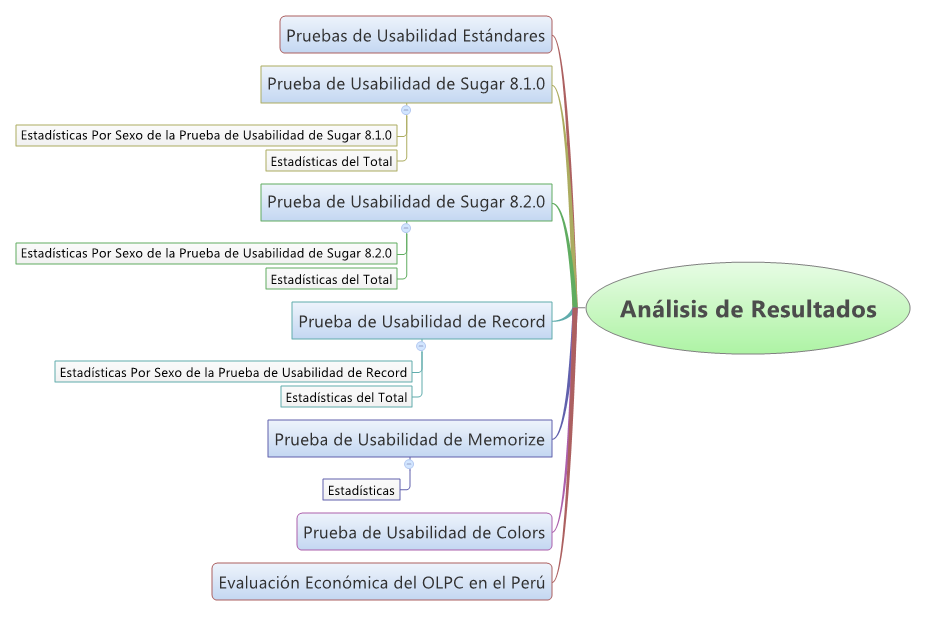
\includegraphics[scale=0.50]{./img/MapaMental/capitulo061.png}
	\caption{Mapa Mental del Cap�tulo de An�lisis de Resultados}
	\label{Mapa Mental del Capitulo de An�lisis de Resultados}
\end{figure}


% ----------------------------------------------
\section{Desarrollo de Pruebas de Usabilidad Est�ndares}
\label{section.DesarrollodePruebasdeUsabilidadEstandares}

El total de las pruebas de usabilidad realizadas de forma satisfactoria\footnote{No se cuentas las pruebas fallidas o mal ejecutadas por problemas de los equipos o por demasiado nerviosismo del usuario por ejemplo el exceso de sudoraci�n en las manos luego de una actividad de educaci�n f�sica.} se muestra en la Tabla \ref{CuadroDePruebasDeUsabilidad}. 

\begin{table}[ht]
\footnotesize
	\centering
	\begin{tabular}{|m{7cm}|m{1.2cm}|m{1.2cm}|}
		\hline	
 & \textbf{Ni�os} & \textbf{Ni�as}\\\hline
\multicolumn{3}{|m{9.4cm}|}{OLPC Sugar Build 703 Rel. 8.1.0} \\\hline
Test de Usabilidad de Sugar Desktop	& 6	& 6\\\hline
Test de Usabilidad de Grabar & 6 & 6\\\hline
Test de Usabilidad de Memoria & 3 & 3\\\hline
Test de Usabilidad de Pintar & 1 & 1\\\hline
\multicolumn{3}{|m{9.4cm}|}{OLPC Sugar Build 656 Rel. 7.2.0} \\\hline
Test Piloto de Usabilidad de Turtle Art &	1 & 1\\\hline
\multicolumn{3}{|m{9.4cm}|}{ClassMate Ubuntu} \\\hline
Test Piloto de Usabilidad de Turtle Art &	1 &	1\\\hline
\multicolumn{3}{|m{9.4cm}|}{OLPC Sugar Build 767 Rel 8.2.0} \\\hline
Test de Usabilidad de Sugar Desktop	& 6 &	6\\\hline
Totales	& 24 &	24\\\hline
		\end{tabular}
	\caption{Cuadro de Pruebas de Usabilidad}
	\label{CuadroDePruebasDeUsabilidad}
\end{table}

El an�lisis de las pruebas de usabilidad se realizar�n por cada prueba.
Las pruebas de usabilidad fueron registradas por medio de filmaciones digitales. Cada uno de estos videos fue procesado en las Tablas \ref{TiempoparaSugar081}, \ref{TiempoparaSugar082}, \ref{TiempoparaRecord}, \ref{TiempoparaMemorize} se tiene la descripcion de cada prueba de usabilidad el tama�o, el tipo de compresi�n usado fue wmv1\footnote{WMV no se construye s�lo con tecnolog�a interna de Microsoft. Desde la versi�n 7 (WMV1), Microsoft ha utilizado su propia versi�n no estandarizada de MPEG-4. El v�deo a menudo se combina con sonido en formato Windows Media Audio. Extraido de http://es.wikipedia.org/wiki/Windows\_Media\_Video 12/10/2009} se  intent� usar el formato ogv\footnote{Ogg encapsula datos comprimidos (e incluso sin comprimir) y permite la interpolaci�n de los datos de audio y de v�deo dentro de un solo formato conveniente. Extraido de http://es.wikipedia.org/wiki/Ogg 12/10/2009. P�gina del Proyecto http://www.xiph.org/ogg/ 12/10/2009.} pero se tuvo muchas p�rdidas en los cuadros. Cada uno de las pruebas se muestran en el Anexo \ref{section.anexo.10} en un despliegue de 12 cuadros.
% ----------------------------------------------//
\section{Desarrollo de Prueba de Usabilidad de Sugar 8.1.0}
\label{section.Desarrollo de Prueba de Usabilidad de Sugar 8.1.0}

\section{Desarrollo de Prueba de Usabilidad de Record}
\label{section.DesarrollodePruebasdeUsabilidadEstandares}

\subsection{Descripci�n del Modelo y Procedimiento}
\label{subsection.Descripci�n.del.Modelo}

